\documentclass[aps,twocolumn,secnumarabic,balancelastpage,amsmath,amssymb,nofootinbib, floatfix]{revtex4-1}
\usepackage[russian]{babel}
\usepackage{graphicx}      % tools for importing graphics
\usepackage{float}
\usepackage{epsf}          % old package handles encapsulated postscript issues
\usepackage{bm}            % special bold-math package. usge: \bm{mathsymbol}
\usepackage[colorlinks=true]{hyperref}  % this package should be added after 
\usepackage[inkscapelatex=false]{svg}
\usepackage{subfigure}
	%%%%%%%%%%%%%%%%%%%%%%%%%%%%%%%%%%%%%%%%%%%%%%%%%%%%%%%%%%%%%%%%%%%
	% And now, begin the document...
	%%%%%%%%%%%%%%%%%%%%%%%%%%%%%%%%%%%%%%%%%%%%%%%%%%%%%%%%%%%%%%%%%%%
	\begin{document}
	\title{Моделирование голограммы\\}
	\author{Лузгина А.А.}
	\email{luzgina.aa@phystech.edu}
	\homepage{\\https://old.mipt.ru/education/chair/physics/laboratornyy-praktikum/} %If you don't have one, just comment out this line.
	\date{\today}
	\affiliation{Ноутбук фирмы "Maxwell equations"}
	
	
	\begin{abstract}
		Работа представляет программную модель записи и восстановления голограмм Габора основанную на численном моделировании интерференции и дифракции. Разработаны модули генерации геометрии объекта (сетка точек), расчёта интерференционной картины и восстановления изображения через FFT. Для точечных источников продемонстрирована корректная симуляция: интерференционные паттерны и изменение изображения при смене ракурса. Для объёмных объектов выявлены ошибки, связанные с расчётом фаз, предложено решение через декомпозицию на точечные источники. Результаты подтверждают возможность моделирования голограмм Габора и важность точного учёта фазовых данных. 
	\end{abstract}
	
	\maketitle
	
	
	
	
	%%%%%%%%%%%%%%%%%%%%%%%%%%%%%%%%%%%%%%%%%%%%%%%%%%%%%%%%%%%%%%%%%%


%%%%%%%%%%%%%%%%%%%%%%%%%%%%%%%%%%%%%%%%%%%%%%%%%%%%%%%%%%%%%%%%%%

		\section{Введение}  

Голография — это метод записи и воспроизведения трёхмерных изображений объектов. В отличие от традиционных методов получения изображений, которые фиксируют только интенсивность света, голография позволяет записывать как амплитуду, так и фазу световой волны, что делает возможным восстановление полного трёхмерного изображения объекта.  

Проект "Симуляция голограммы" направлен на создание программной модели, которая позволяет:  \begin{enumerate}
\item Рассчитывать запись голограммы в зависимости от заданной геометрии объекта.  
\item Визуализировать восстановленное изображение с учётом положения наблюдателя.  
\end{enumerate}

\section{Теоретическая справка} 

\subsection{Принципы голографии} 

Голография основывается на интерференции и дифракции света.  
\begin{enumerate}
	\item \textbf{Запись голограммы}:\\
	Для записи голограммы используют два когерентных световых пучка:  
	\begin{enumerate}
		\item \textbf{Опорный пучок}: когерентный свет, освещающий фотопластинку.  
		\item \textbf{Объектный пучок}: свет, отражённый от объекта.  
	\end{enumerate}
На фотопластинке создаётся интерференционная картина, где записывается амплитудно-фазовая информация об объекте.  
	\item \textbf{Восстановление изображения}:  
	При освещении голограммы опорным пучком происходит дифракция света, в результате чего наблюдатель видит трёхмерное изображение объекта.  
	
\end{enumerate}

\subsection{Интерференция и запись голограммы}

Формула интерференции двух когерентных пучков света:  
\[
I(x, y) = |E_r(x, y) + E_o(x, y)|^2,
\]  
где \(E_r(x, y)\) — вектор опорной волны, \(E_o(x, y)\) — вектор волны, отражённой от объекта.  

Разложив эту формулу, получим:  
\[
I(x, y) = |E_r|^2 + |E_o|^2 + 2 \text{Re}(E_r E_o^*),
\]  
где \(E_o^*\) — комплексное сопряжение амплитуды объектной волны.  

Таким образом, интенсивность света в точке зависит не только от амплитуд, но и от фазовых сдвигов между волнами.  

\subsection{Восстановление изображения}

При восстановлении изображения дифракция света на голограмме формирует три пучка:  
\begin{enumerate}
	\item \textbf{Нулевой-дифракционный пучок} (нулевой порядок): содержит лишь интенсивностную информацию.  
	\item \textbf{Пучок +1 порядка}: создаёт изображение объекта.  
	\item \textbf{Пучок -1 порядка}: формирует виртуальное изображение.  
\end{enumerate}
\subsection{Голограмма Габора }

В проекте моделируется голограмма Габора — один из первых методов записи объемных изображений (придуман в 1962г. Юрием Николаевичем Габором). При этом голограмма записывается и восстанавливается с использованием одного и того же источника света.  

\section{Описание реализации проекта } 

\subsection{Архитектура проекта }

Проект состоит из нескольких модулей, каждый из которых отвечает за определённую часть симуляции:  
\begin{enumerate}
\item[-]\textbf{Генерация геометрии объекта}:  
Модуль `geometry` отвечает за задание формы объекта, разбиение его поверхности на сетку точек и проверку корректности геометрии.  

\item[-]\textbf{Запись голограммы}:  
Модуль `hologram\_prep` рассчитывает интерференционную картину, создаваемую объектным и опорным пучками, и сохраняет её в виде матрицы интенсивностей.  

\item[-]\textbf{Восстановление изображения}:  
Модуль `calculate\_visible\_field` позволяет восстанавливать видимое изображение объекта с учётом положения наблюдателя.  

\item[-]\textbf{Визуализация}:  
Используется библиотека OpenGL для отображения восстановленного изображения.  
\end{enumerate}
\subsection{Этапы работы} 
\begin{enumerate}
	\item Генерация геометрии объекта  
	
	Объект задаётся в виде набора поверхностей, каждая из которых представлена четырьмя вершинами:  
	\[
	\text{vertexes} = \{\{P_1, P_2, P_3, P_4\}, \dots\},
	\]  
	где \(P_i = (x, y, z)\).  
	
	Пример генерации объекта — плоского квадрата:  
	\begin{verbatim}cpp
		
		
	std::vector<std::vector<Point>> vertexes = {
	{ {0, 0, 0}, {1, 0, 0}, {0, 1, 0}, {1, 1, 0}}
	};
	obj_geometry geometry(1e-6, {100, 100}, 
			vertexes);
	geometry.calculate_points();
	\end{verbatim}
	\item Запись голограммы  
	Запись голограммы моделируется путём расчёта интерференционной картины. 
	\begin{verbatim}
std::string name_from = "file_with_geometry";
std::string name_to = 
	"file_where_to_save_intensity.txt";
double width = 10.0;
double height = 10.0;
double scale = 1e-6;
std::vector<unsigned int> np = {1024, 1024};
obj_plate plate(scale, np, width, height);
plate.readDataFromFile(name_from);
plate.calculate_intensity_matrix();
plate.saveIntensityToFile(name_to);
	\end{verbatim}
	\item Восстановление изображения  
	
	Восстановление голограммы выполняется методом быстрого преобразования Фурье (FFT). Использовалась библиотека `fftw3`. 
	\begin{enumerate}
		\item[-] \textbf{FFT} позволяет выделить пучок +1 порядка, содержащий информацию об объекте. 
		\item[-] Результат восстанавливается в виде матрицы интенсивностей, которая затем отображается.  
	\end{enumerate}
	Пример восстановленного изображения:
	\begin{verbatim}
		std::string name_from = "file_with_intensity";
		v_plate = obj_visible_plate(1e-6);
		v_plate.read_intensity_matrix(name_from);
		...
		while(...){ //main loop
			...
			v_plate.update_visible_matrix(cameraPos.x,
			 cameraPos.y, cameraPos.z);
			...
		}
	\end{verbatim}	
\end{enumerate}
\subsection{Результаты}
(Получилось мало чего, но мы честно пытались, а еще мысли что делать дальше)
\begin{figure}[htbp]
	\centering
	\subfigure[интерференционная картина для точеченого источника]{
		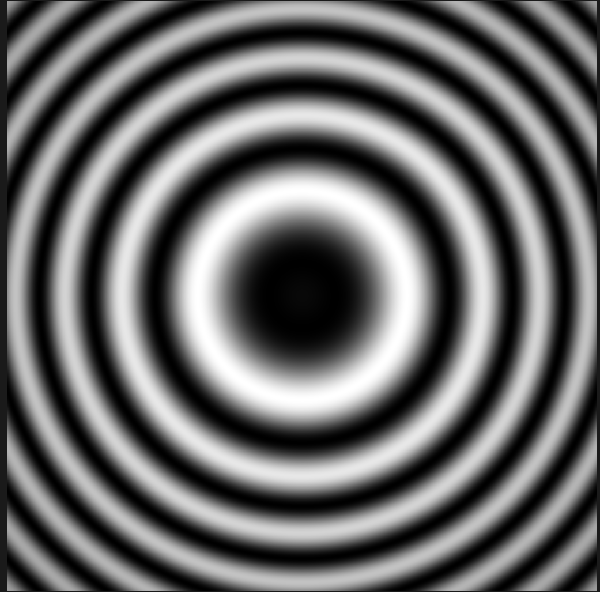
\includegraphics[width=0.21\textwidth]{images/point_interf.png}
		\label{subfig:point_interf}
		%\caption{fig1}
	}
	\quad
	\subfigure[]{
		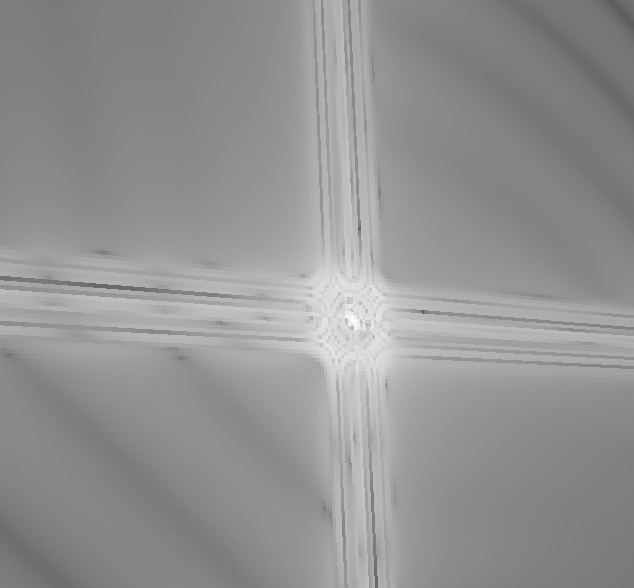
\includegraphics[width=0.21\textwidth]{images/point1.png}
		\label{subfig:point1}
		%\caption{fig1}
	}
	\quad
	\subfigure[]{
		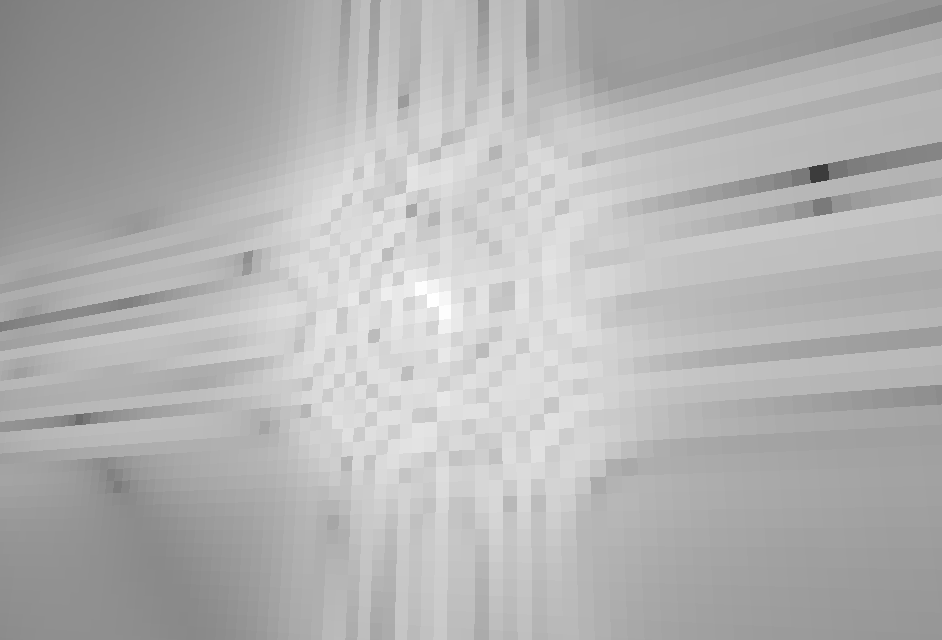
\includegraphics[width=0.21\textwidth]{images/point2.png}
		\label{subfig:point2}
	}
	\quad
	\subfigure[]{
		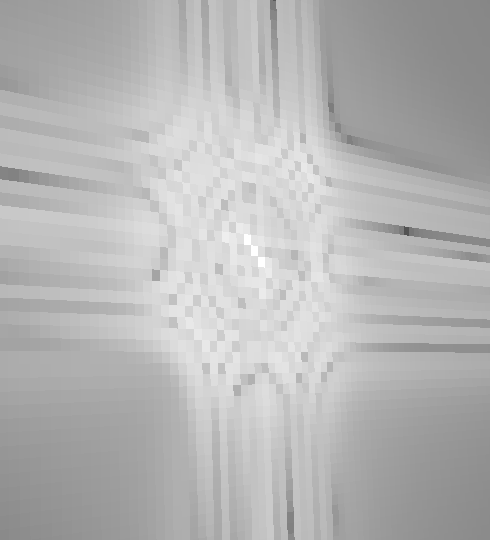
\includegraphics[width=0.21\textwidth]{images/point4.png}
		\label{subfig:point3}
	}
	\caption{Интерференционная картина, которая бы была на транспаранте и изображение точеной голограммы с разных ракурсов (можно заметить, что немного картины интенсивностей, который бы видел человеческий глаз меняются)}
	\label{fig:point_hologram}
\end{figure}
\begin{figure}[htbp]
	\centering
	\subfigure[геометрия, расчитанная в этом варианте]{
		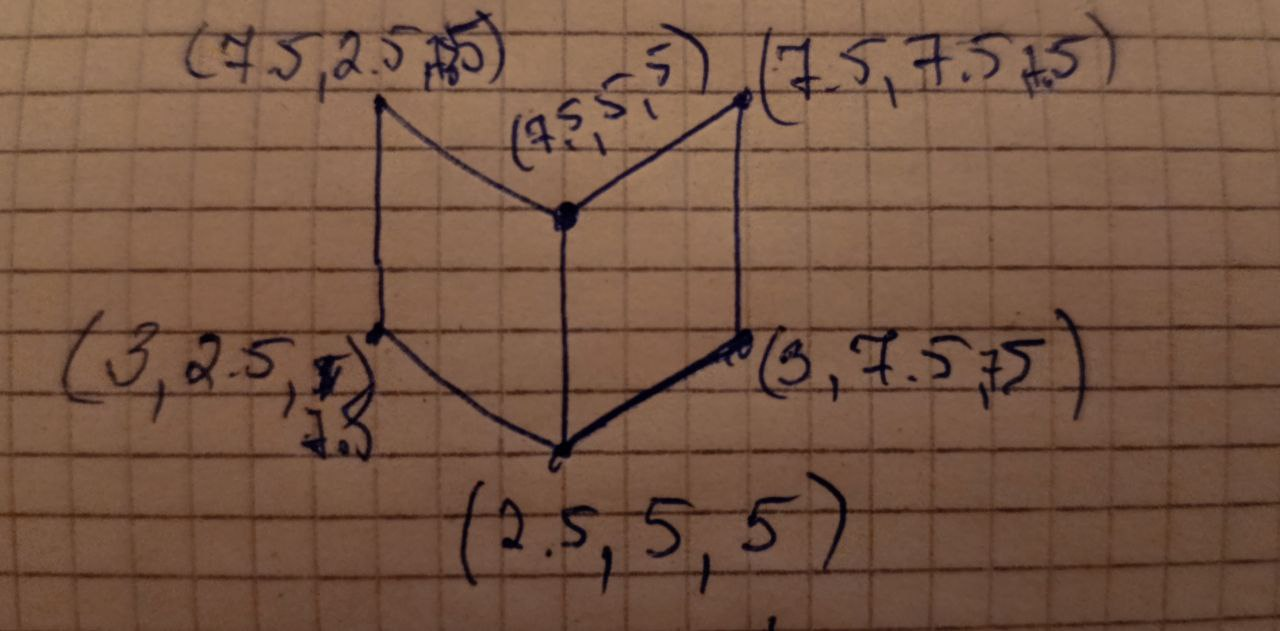
\includegraphics[width=0.45\columnwidth]{images/book.jpeg}
		\label{subfig:book}
		%\caption{fig1}
	}
	\quad
	\subfigure[интерференционная картина для точеченого источника]{
		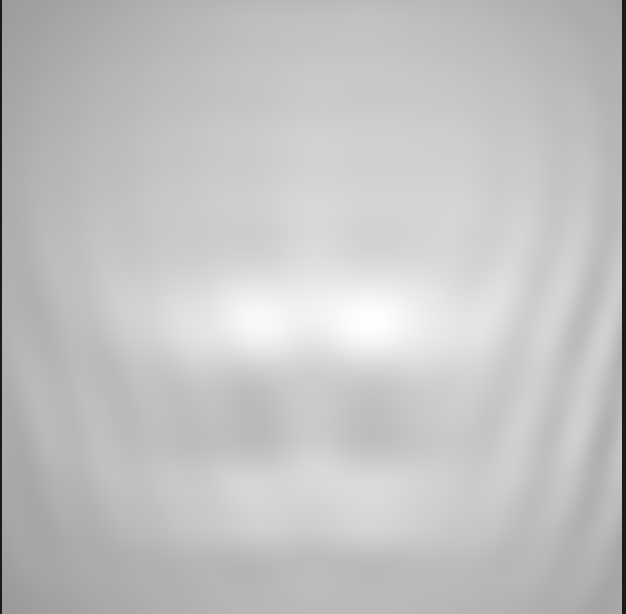
\includegraphics[width=0.45\columnwidth]{images/sq_interf.png}
		\label{subfig:sc_interf}
		%\caption{fig1}
	}
	\quad
	\subfigure[]{
		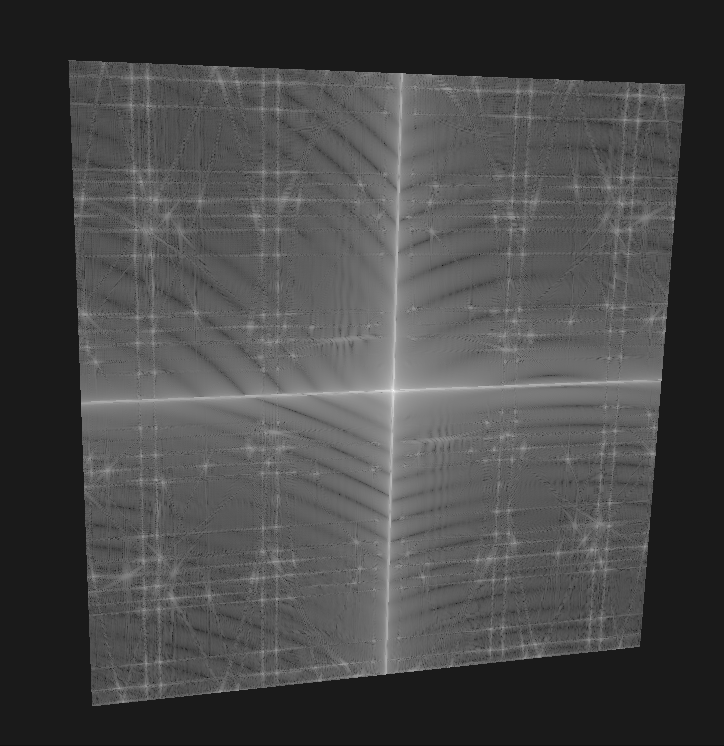
\includegraphics[width=0.45\columnwidth]{images/screen1.png}
		\label{subfig:screen1}
	}
\quad
\subfigure[]{
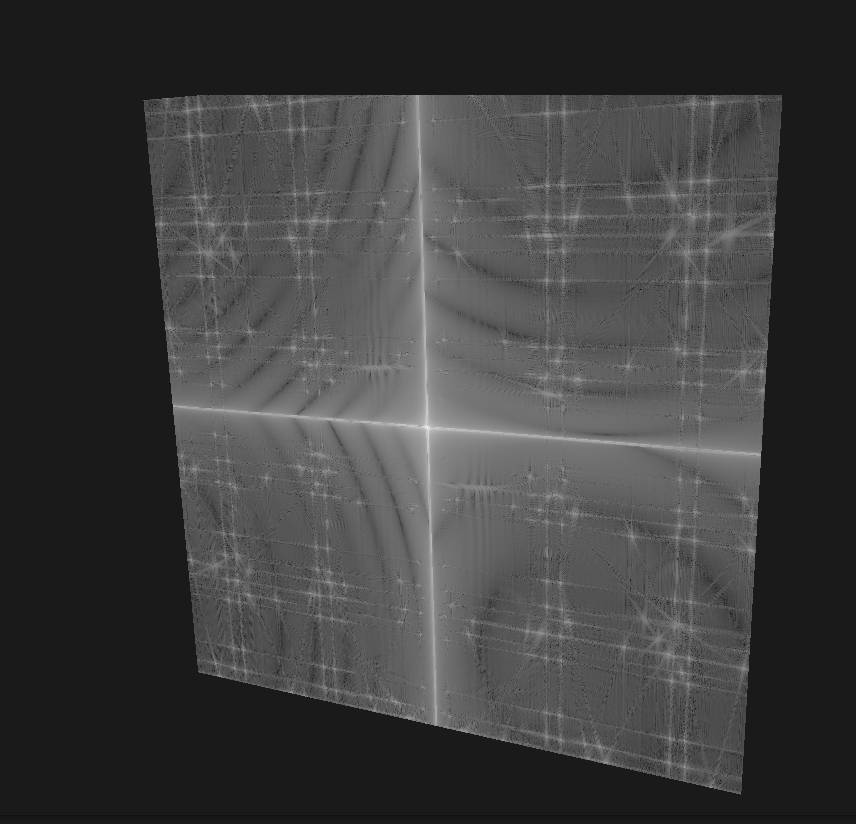
\includegraphics[width=0.45\columnwidth]{images/sq_2.png}
\label{subfig:sq_2}
}
	\caption{Геометрия, интерференционная картина, которая бы была на транспаранте и изображение объемной голограммы с разных ракурсов (можно заметить, что немного картины интенсивностей, который бы видел человеческий глаз меняются)}
	\label{fig:book_hol}
\end{figure}
\section{Обсуждение результатов}
Скорее всего, моделирование не получилось для объемного источника из-за того, что где-то появилась ошибка в задании фазы. \\ 
Один из вариантов, для исправления этой ситуации, это решать задачу путем фурье преобразований. Для точечного источника результат известен, а так как объемное изображение можно собрать из множества точек, то таким образом можно так же моделировать голограмму.
\section{ Итоги и выводы  }

1. Реализована программная модель записи и восстановления голограммы.  
2. Использованы методы численного моделирования, такие как FFT, для восстановления изображения.  
3. Полученные результаты демонстрируют возможность симуляции голограммы Денисьюка с учётом положения наблюдателя.  

\section{Ссылки на литературу}  

1. Hecht, E. \textbf{Optics}, Fifth Edition. Pearson Education, 2017.  
2. Бутиков Е. И. \textbf{Оптика: Учебное пособие}. 3-е изд. Санкт-Петербург: Лань, 2016.  

\section{Приложения}  
Код проекта расположен по \href{https://github.com/ArinaLuzgina/holographySimulation}{ссылке}.
\end{document}
